The following is extracted from our initial report \cite{init}
\subsection{Objectives}
	Our primary objective is to create a system which can take as input a road system
	and a journey matrix and produce overall statistics about journey times between the entry/exit points
	and allow us to change something about the network or the demand and produce new statistics for
	comparison. Our aim is to model individual vehicle movements as realistically as possible, taking 
	into account driver type, vehicle type, car following behaviour, lane switching behaviour and junction
	modelling. The system will output statistics and raw data for each vehicle journey which could be
	further analysed using a statistical analysis tool such as SPSS.
\\ \\
	\subsection{Project Roadmap}
	
	\begin{description}
		\item[Stage 1] Decide on a model for traffic simulation.
		\item[Stage 2] Research existing implementations.
		\item[Stage 3] Develop architecture for the system(see \ref{secarch}).
		\item[Stage 4] Decide on a development methodology and technology to build the system.
		\item[Stage 5] Build the Core. The Core consists of the building blocks of the simulation i.e. Roads, Junctions, Vehicles.
		\item[Stage 6] Build Services around the Core. Services control the running of simulation, traffic light scheduling, populating the demand matrix, gathering and reporting statistics.  
		\item[Stage 7] Build a Client. The Client is a User Interface to the system. The Client allows the user to access system services.
		\item[Stage 8] Final report.
		\\
	\end{description}
	
	\subsection{Design}
		\label{secarch}
	The Core of the system consists of the following entities
	\begin{enumerate}
		\item Vehicle: This describes an entity travelling on the network. Vehicles have speed, acceleration, a maximum speed and behaviour. The vehicle is configured with a Source node and Destination node when it's added to the simulation. 
		
		\item Node: A node is the base component of our road model. A node represents a cell in the cell automata model. Each node can accommodate a vehicle of length one. A sequence of nodes forms a lane.
		
		\item Lane: A lane is a sequence of nodes that represents a lane on a road. Each lane supports traffic in one direction.
		
		\item Road: A road is comprised of one or more lanes. They allow travel in one direction, from a source, to a sink.
		
		\item Junctions: Junctions allow for transferring traffic between two or more road segments. In our base model we will allow each junction to have four interfaces (North, East, South \& West). Each interface has a junction entry and an exit mapping onto roads to build the network.
	\end{enumerate}
	The Services provided by the system are as follows
	\begin{enumerate}
		\item Control the running of the simulation by modifying the tick of the global clock.
		
		\item Configure the schedule of the traffic signals at the different junctions.
		
		\item Populate the Demand Matrix which specifies the density of traffic between two destinations.
		
		\item Mechanism to gather statistics on average journey time, average speed, etc.
	\end{enumerate}
	
	\subsubsection{Routing configuration}
		Each junction maintains a routing table to move vehicles to the appropriate junction exit towards their destination. These routing tables will be initially static, but may be made to function dynamically as we increase the sophistication of our network.
		
	\subsubsection{Policy configuration}
	
	\begin{enumerate}
		\item The user can supply a demand matrix to the simulation. This demand matrix will determine the relative frequency of vehicles travelling between any two destinations. A multiplier will then be calculated using other available information to determine the absolute values.
		\item The user can control the scheduling of traffic signals at junctions.
	\end{enumerate}
    \subsection{UML}
    \subsubsection{Use case diagram}
    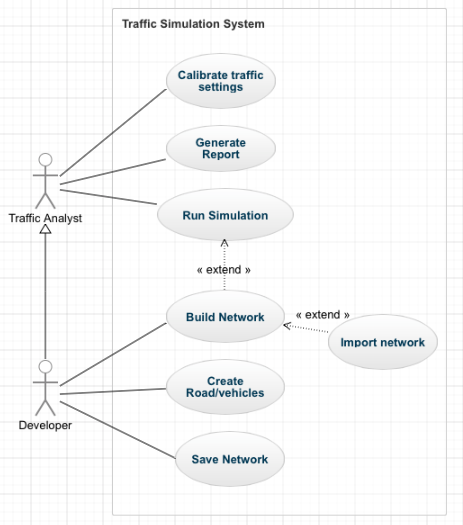
\includegraphics[scale=0.7]{./images/usecase.png}
    
    
\textit{Run Simulation} \\
The Traffic analyst chooses to run the simulation. The system starts the simulation and provides visual feedback while it is running. The traffic analyst can stop or start the simulation whenever he/she decides to do. When the traffic analyst decides to stop the simulation the, system stops running the simulation and keeps the model in this state, allowing the traffic analyst to subsequently start or run the simulation from where it was stopped.\\


\textit{Calibrate Traffic settings} \\
The Traffic analyst or developer chooses to adjust the traffic settings. The system displays available settings to change. Using the graphical interface widgets, the traffic analyst or developer can alters any traffic settings such as; traffic light interval, maximum velocity of vehicles, clock interval, the demand matrix for cars and buses. The system stores the new values of any adjustments or changes made. \\

\textit{Generate report} \\
The traffic analyst chooses to generate a report of the simulation. The system generates the report with all recorded statistics in text format. \\

\textit{Build New Network} \\
The developer chooses to build a new network. The system creates a blank network or alternatively, the developer can choose to Import Network. The system is now ready for another network simulation and calibrating traffic settings. \\

\textit{Create Road/Vehicles} \\
The developer creates new road and lanes, junctions, roundabouts on the network and different vehicles either cars or bus. \\

\textit{Import Network} \\
The system provides a file chooser. The developer finds an existing traffic network file saved on his/her device. The system verifies and loads the existing network into the model. \\

\textit{Save Network} \\
The developer chooses to save the network to the model. The system provides a file chooser to determine where to save. The developer selects an existing file or gives a name for a new network file.\\
 \subsubsection{class diagram}
Road Network class design with vehicle class\\
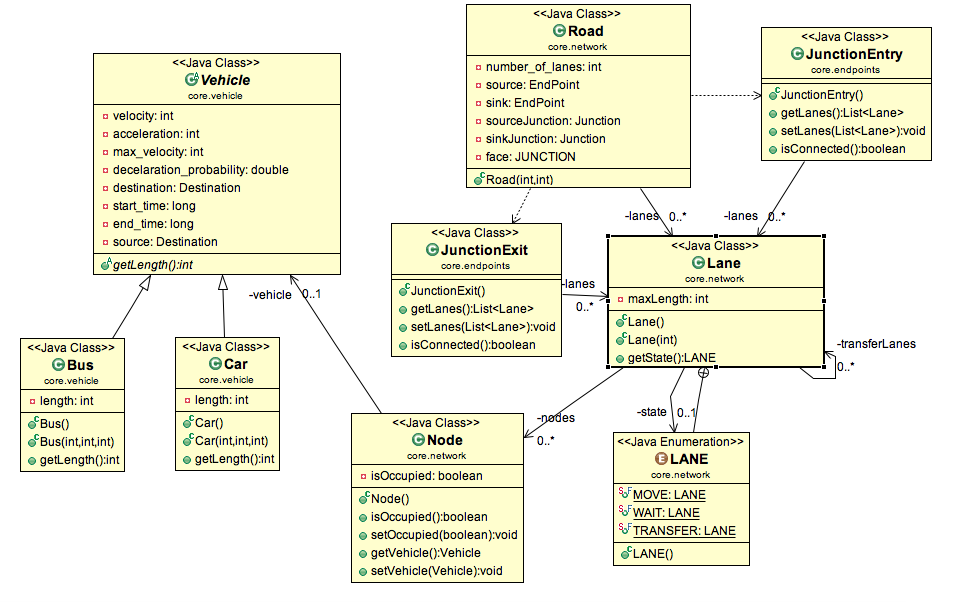
\includegraphics[scale=0.3]{./images/class1.png} ~\\

The above diagram shows the traffic network using links and nodes, the system represents the road on a discrete network of cells, the roads can be vertical, horizontal or even both. It allows different scenarios to be modelled. A junction is simply a road with lanes leading to it in different direction. In this model there are two types of vehicles namely; buses and cars.

\subsubsection{Traffic lights and junctions}
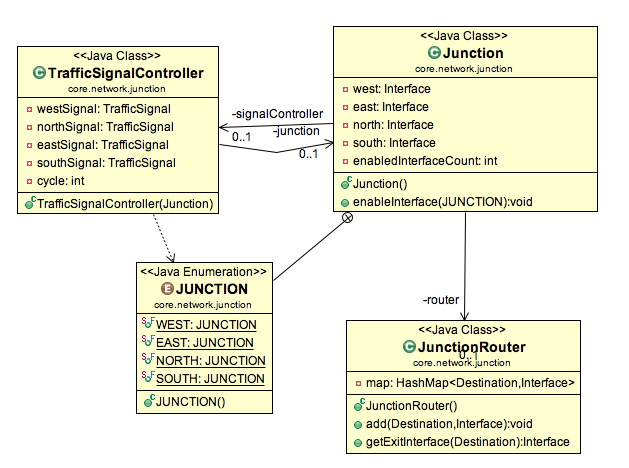
\includegraphics[scale=0.4]{./images/class4.png}


The class diagram above shows the relationship between the traffic signal controller and the junctions in all four directions; north, south, east and west. This function defines the basis of the network, as the vehicles will follow the instructions given by the traffic signal control at each junction in order to safely get to their various destinations

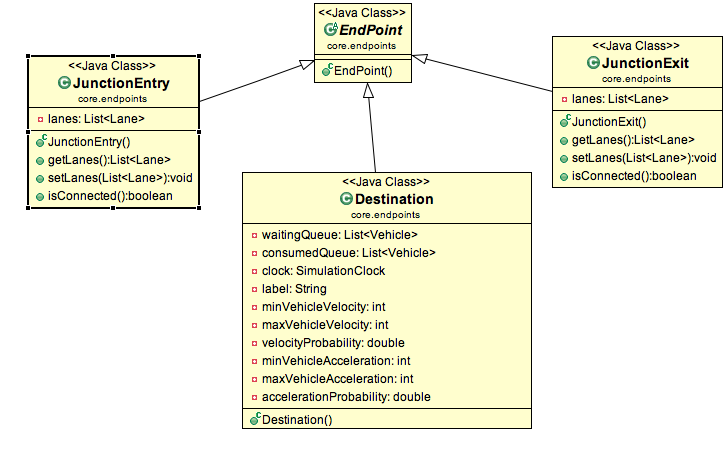
\includegraphics[scale=0.4]{./images/class3.png}

\subsubsection{Sequence Diagram}

Sequence diagrams are sorts of interaction diagram that show the flow of messages through a framework as a specific function is being executed. The sequence diagram below describes the sequence of events that occur during a simulation run. It shows a single interval, and during normal use, this sequence would be repeated for the duration of the simulation. \\
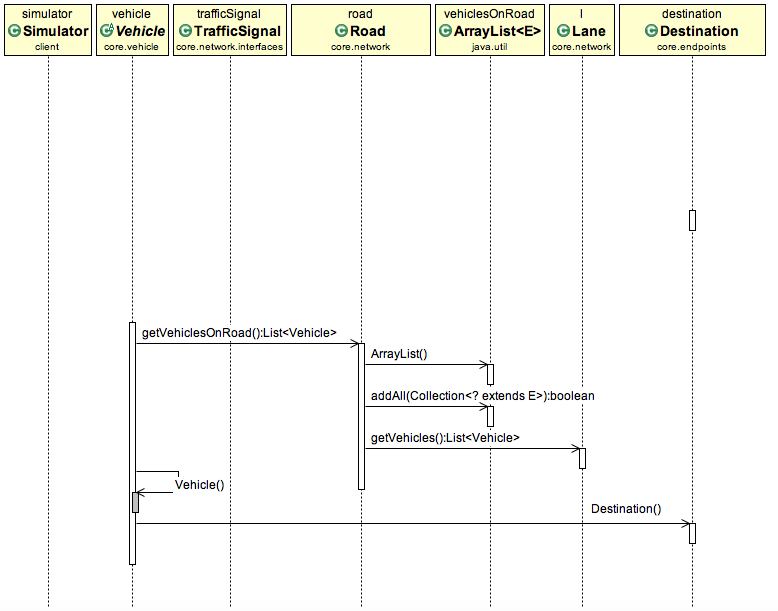
\includegraphics[scale=0.4]{./images/interaction.png}








	